\documentclass[]{exam}

\usepackage{amsmath}
\usepackage{amssymb}
\usepackage{tikz}
\usepackage{tabularx}
\tikzstyle{vertex}=[circle,fill=black!25,minimum size=17pt,inner sep=0pt]

\pagestyle{empty}
\extrawidth{.5in}

\def\bonuson{\renewcommand\partlabel{*(\thepartno)}}
\def\bonusoff{\renewcommand\partlabel{(\thepartno)}}

\begin{document}
  \begin{center}
    \fbox{\fbox{\parbox{5.5in}{\centering Answer the questions in the spaces
    provided on the question sheets. If you run out of room for an answer,
    continue on a separate sheet of paper.}}}
  \end{center}

  \begin{questions}
    \question Define the set $A = \{\ r,\ o,\ t,\ p,\ c\ \}$ and $B = \{\
      discrete,\ math,\ proof,\ proposition\ \}$. Define the relation $R
      \subseteq A \times B$ such that (letter, word) is in the relation if that
      letter occurs somewhere in the word. Draw the arrow diagram and the matrix
      representation for each relation.
      \vspace{\stretch{1}}

    \question The domain of relation $D$ is $\{\ 2,\ 3,\ 12,\ 16,\ 27,\ 48\ \}$.
      For $x, y$ in the domain, $xDy$ if $y$ is an integer multiple of $x$. Draw
      the arrow diagram and the matrix representation for each relation.
      \vspace{\stretch{1}}

    \question Consider the following relation $F$. The domain of the relation
      $F$ is all Facebook users. For $x,y$ in the domain, $xFy$ if $x$ and
      $y$ are Facebook friends. Furthermore, $xFy \rightarrow yFx$. 

      \begin{parts}
        \part List all properties of the relation $F$.
          \vspace{\stretch{1}}

        \part Read about ``\emph{Six degrees of separation}'' on Wikipedia. What
          is the implication of this claim for the relation $F$ described above?
          \vspace{\stretch{1}}

        \part Now read this article
          \texttt{https://research.fb.com/blog/2016/02/three-and-a-half-degrees-of-separation/}.
          What does this mean for you?
          \vspace{\stretch{1}}
        \end{parts}

    \newpage

    \question Define the directed graph $G$ as follows:

      \bigskip

      \begin{center}
        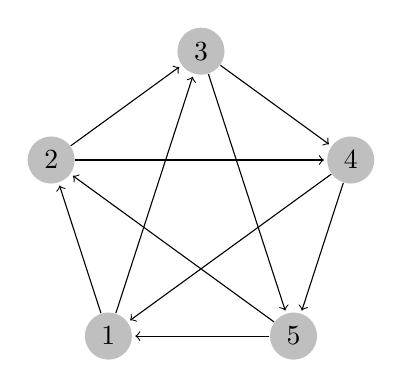
\begin{tikzpicture}[shorten >=1pt,->]
          \foreach \name/\angle/\text in {P-1/234/1, P-2/162/2, 
                                          P-3/90/3, P-4/18/4, P-5/-54/5}
            \node[vertex,xshift=6cm,yshift=.5cm] (\name) at (\angle:2cm) {$\text$};
          \foreach \from/\to in {1/2,2/3,3/4,4/5,5/1,1/3,2/4,3/5,4/1,5/2}
            \draw (P-\from) -- (P-\to);
        \end{tikzpicture}
      \end{center}

      \bigskip

      \begin{parts}
        \part Classify each of the following sequences of vertices as either a
          \emph{walk} in $G$ or \emph{not a walk} in $G$. If a sequence, $w$
          represents a walk in $G$, characterize the walk as an \emph{open
          walk}, \emph{closed walk}, \emph{trail}, \emph{circuit}, \emph{path}
          or \emph{cycle}, being as specific as possible.

          \begin{subparts}
            \begin{tabularx}{\linewidth}{XcXcXcX}
              \subpart $\langle 1,\ 2,\ 4,\ 5,\ 2\rangle$
                \begin{solution}
                  trail
                \end{solution} &&
              \subpart $\langle 1,\ 3,\ 5,\ 2,\ 4,\ 1\rangle$
                \begin{solution}
                  cycle
                \end{solution} &&
              \subpart $\langle 1,\ 2,\ 3\rangle$
                \begin{solution}
                  path
                \end{solution} &&
              \subpart $\langle 3,\ 5,\ 1,\ 2,\ 4,\ 1,\ 3\rangle$
                \begin{solution}
                  circuit
                \end{solution}
            \end{tabularx}
          \end{subparts}

          \vspace{\stretch{1}}

        \part For each of the following, find a walk in $G$ that satisfies the
          requirements specified.

          \begin{subparts}
            \begin{tabularx}{\linewidth}{XcXcX}
              \subpart cycle of length 3
                \begin{solution}
                  ~\newline
                  $\langle 1,\ 3,\ 5,\ 1\rangle$
                \end{solution} &&
              \subpart trail of length 8
                \begin{solution}
                  ~\newline
                  $\langle 1,\ 2,\ 3,\ 4,\ 5,\ 1,\ 3,\ 5,\ 2\rangle$
                \end{solution} &&
              \subpart path of length 4 starting at 5 and ending at 3
                \begin{solution}
                  ~\newline
                  $\langle 5,\ 2,\ 4,\ 1,\ 3\rangle$
                \end{solution}
            \end{tabularx}
          \end{subparts}

          \vspace{\stretch{1}}
      \end{parts}
  \end{questions}
\end{document}
